\section{Diagramy klas}

W poniższym rozdziale zaprezentowane zostały diagramy klas. Ukazano uproszczoną strukturę systemu ze względu na podział na klasy. Podstawowym kryterium podziału jest program, w którym znajdują się dane klasy. W pierwszej części przedstawiono klasy użyte w aplikacji klienta, w drugiej natomiast wykorzystane w serwisie internetowym.

\subsection {Aplikacja klienta}
Poniżej przedstawiono diagram klas znajdujących się w aplikacji klienta. Klasy ApplicationForm i Podglad są oknami Windows Form. Klasy ServerHandler oraz ServerConnection są wykorzystywane do połączenia z serwerem za pomocą biblioteki SignalR. Klasa Spy udostepnia za to metody odpowiedzialne za tworzenie zrzutu ekranu, pobieranie listy otwartych stron oraz aktywnych procesów.

\begin{figure} [!ht]
    \centering
    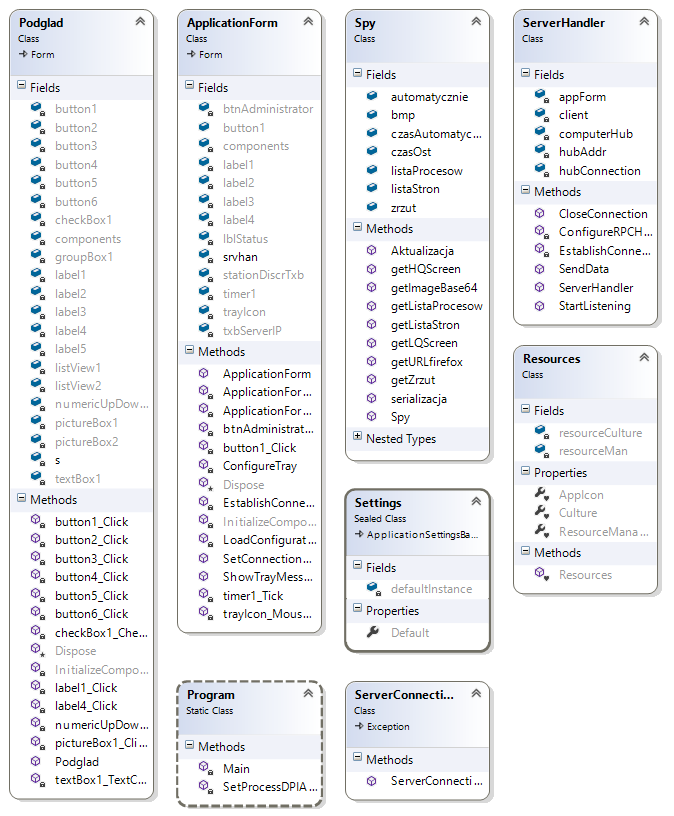
\includegraphics[height=10cm,width=9cm]{diagramklas_klient}
    \caption{Diagram klas - aplikacja klienta}
    \label{fig:my_label}
\end{figure}

\subsection{Serwer}

Poniżej natomiast znajdują się diagramy klas w aplikacji serwera. Zostały one podzielone na dwie części, ze względu na ilość klas, jaka została użyta. Klasy Computer, Classroom, ClassroomPermision oraz User zostały napisane do obsługi bazy danych zgodnie z metodą CodeFirst przy wykorzystaniu Entity Framework. Oprócz tego znajdują się kontrolery odpowiedzialne za każdy widok oraz same widoki. Dodatkowo są zaimplementowane huby potrzebne do połączenia z klientami.

\begin{figure} [!ht]
    \centering
    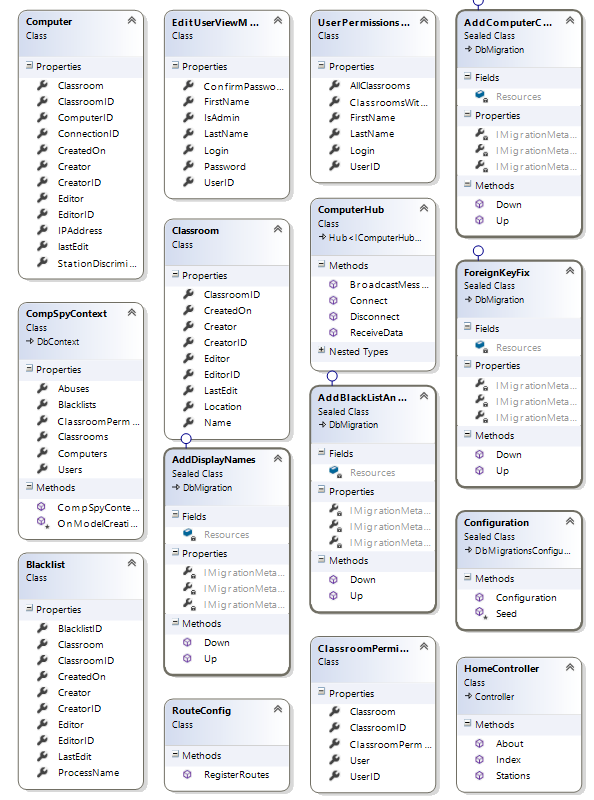
\includegraphics[height=12cm,width=12cm]{diagramklas_serwer1}
    \caption{Diagram klas - aplikacja serwera cz. 1}
    \label{fig:my_label}
\end{figure}
\newpage
W modelach oprócz tych klas związanych z bazą danych znajdują się jeszcze klasy Abuse i Blacklist. Natomiast jeśli chodzi o widoki, to zostały podzielone na kategorie: Account, Classrooms, Computers, Home, Shared, Suirvalance oraz User.

\begin{figure} [!ht]
    \centering
    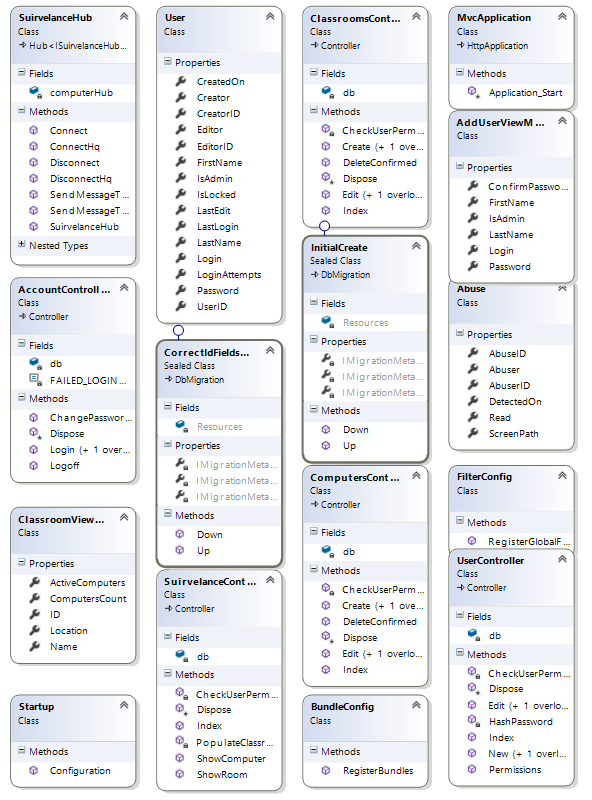
\includegraphics[height=12cm,width=12cm]{diagramklas_serwer2}
    \caption{Diagram klas - aplikacja serwera cz. 2}
    \label{fig:my_label}
\end{figure}